\usetikzlibrary{shapes, arrows.meta, positioning, fit}

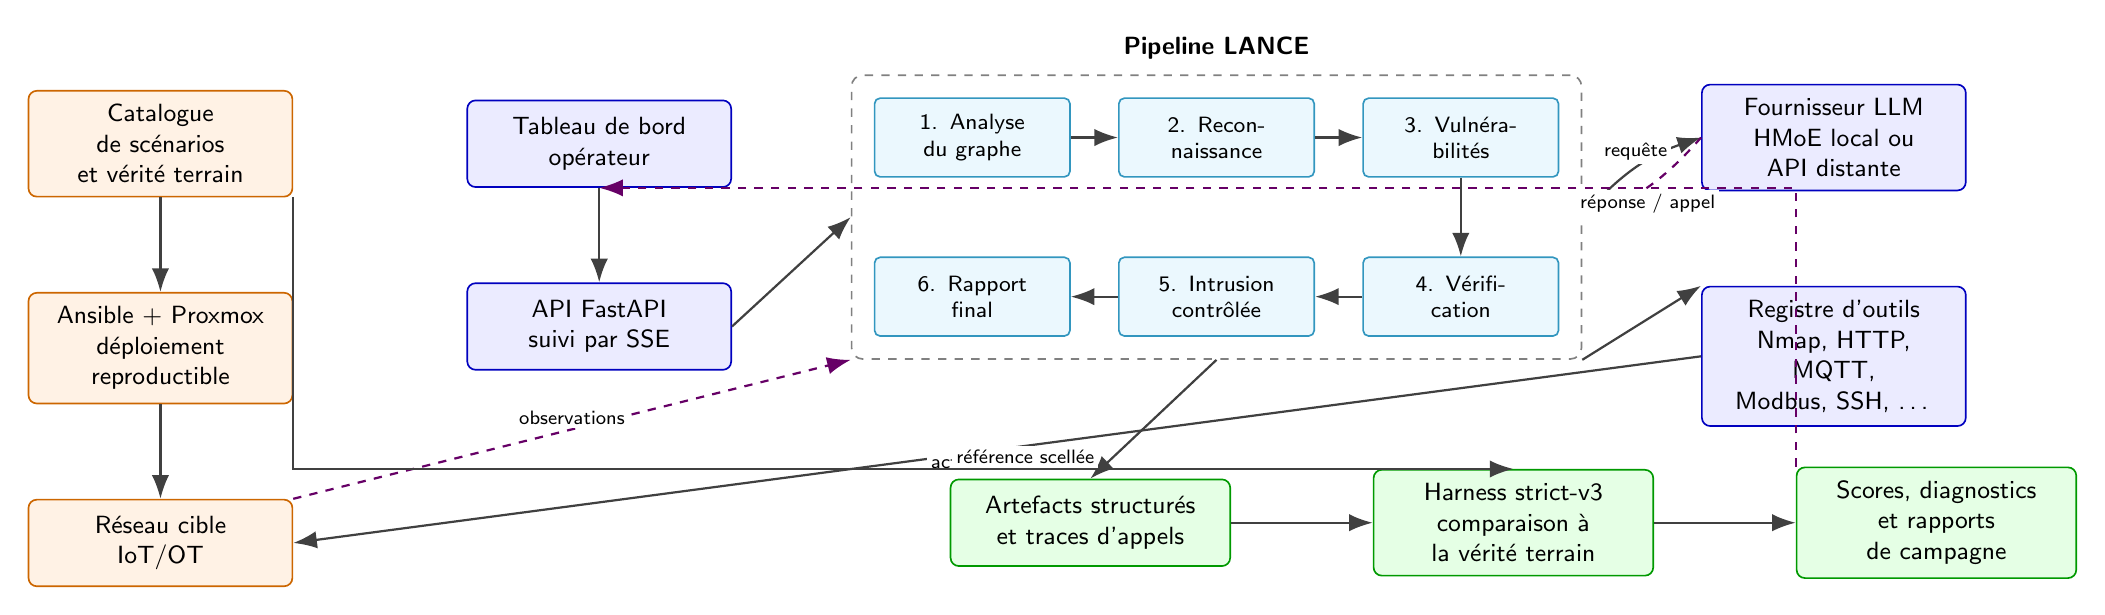
\begin{tikzpicture}[
  font=\sffamily\small,
  >={Latex[length=3mm, width=2.2mm]},
  flow/.style={->, thick, draw=black!75},
  feedback/.style={->, thick, dashed, draw=violet!80!black},
  component/.style={draw=blue!75!black, fill=blue!8, rounded corners=3pt,
    align=center, minimum height=11mm, text width=30mm, inner sep=5pt, semithick},
  phase/.style={draw=cyan!75!black, fill=cyan!8, rounded corners=2pt,
    align=center, minimum height=10mm, text width=22mm, inner sep=4pt, font=\sffamily\footnotesize, semithick},
  external/.style={draw=orange!80!black, fill=orange!10, rounded corners=3pt,
    align=center, minimum height=11mm, text width=30mm, inner sep=5pt, semithick},
  artifact/.style={draw=green!60!black, fill=green!10, rounded corners=3pt,
    align=center, minimum height=11mm, text width=32mm, inner sep=5pt, semithick},
  group/.style={draw=black!50, dashed, rounded corners=4pt, inner sep=8pt, semithick},
  lbl/.style={font=\sffamily\scriptsize, fill=white, inner sep=1.5pt} % Style pour texte sur les flèches
]

  % --- Briques externes (Gauche) ---
  \node[external] (catalogue) {Catalogue de scénarios\\et vérité terrain};
  \node[external, below=12mm of catalogue] (deploy) {Ansible + Proxmox\\déploiement reproductible};
  \node[external, below=12mm of deploy] (target) {Réseau cible\\IoT/OT};

  % --- Interface & API ---
  \node[component, right=22mm of catalogue] (ui) {Tableau de bord\\opérateur};
  \node[component, below=12mm of ui] (api) {API FastAPI\\suivi par SSE};

  % --- Pipeline LANCE ---
  \node[phase, right=18mm of api, yshift=24mm] (p1) {1. Analyse\\du graphe};
  \node[phase, right=6mm of p1] (p2) {2. Recon-\\naissance};
  \node[phase, right=6mm of p2] (p3) {3. Vulnéra-\\bilités};
  \node[phase, below=10mm of p3] (p4) {4. Vérifi-\\cation};
  \node[phase, left=6mm of p4] (p5) {5. Intrusion\\contrôlée};
  \node[phase, left=6mm of p5] (p6) {6. Rapport\\final};
  
  \node[group, fit=(p1)(p2)(p3)(p4)(p5)(p6),
    label={[font=\sffamily\small\bfseries, yshift=2pt]above:Pipeline LANCE}] (pipeline) {};

  % --- Modèle & Outils ---
  \node[component, right=18mm of p3] (model) {Fournisseur LLM\\HMoE local ou API distante};
  \node[component, below=12mm of model] (tools) {Registre d'outils\\Nmap, HTTP, MQTT,\\Modbus, SSH, \ldots};

  % --- Artefacts & Évaluation ---
  \node[artifact, below=18mm of p6, xshift=15mm] (artifacts) {Artefacts structurés\\et traces d'appels};
  \node[artifact, right=18mm of artifacts] (harness) {Harness strict-v3\\comparaison à la vérité terrain};
  \node[artifact, right=18mm of harness] (metrics) {Scores, diagnostics\\et rapports de campagne};

  % --- Liens et Flux ---
  \draw[flow] (catalogue) -- (deploy);
  \draw[flow] (deploy) -- (target);
  \draw[flow] (ui) -- (api);
  \draw[flow] (api.east) -- (pipeline.west);
  
  \draw[flow] (p1) -- (p2);
  \draw[flow] (p2) -- (p3);
  \draw[flow] (p3) -- (p4);
  \draw[flow] (p4) -- (p5);
  \draw[flow] (p5) -- (p6);
  
  \draw[flow, bend left=15] (pipeline.east) to node[lbl, above=1pt]{requête} (model.west);
  \draw[feedback, bend left=15] (model.west) to node[lbl, below=1pt]{réponse / appel} (pipeline.east);
  
  \draw[flow] (pipeline.south east) -- (tools.north west);
  \draw[flow] (tools.west) -- node[lbl, below]{actions bornées} (target.east);
  \draw[feedback] (target.north east) -- node[lbl, above]{observations} (pipeline.south west);
  
  \draw[flow] (pipeline.south) -- (artifacts.north);
  \draw[flow] (artifacts) -- (harness);
  \draw[flow] (harness) -- (metrics);
  
  \draw[flow] (catalogue.south east) |- node[lbl, pos=0.8, above]{référence scellée} (harness.north);
  \draw[feedback] (metrics.north west) |- (ui.south);

\end{tikzpicture}
